\documentclass[aspectratio=169,10pt]{beamer}

\graphicspath{{figures/}}
\usepackage{graphicx}
\usepackage[utf8]{inputenc}

\usepackage[T1,T2A]{fontenc}
\usepackage[main=russian,english]{babel}

\usepackage{cmap}
\usepackage{tikz}
\usepackage{array}
\usepackage{multicol}
\usepackage{booktabs}
\usepackage{csquotes}
\usepackage{amssymb,amsfonts,amsmath}

\usecolortheme{beaver}
\usefonttheme[onlymath]{serif}  % math fonts as in article
\setbeamertemplate{navigation symbols}{}
\setbeamertemplate{footline}[page number]
\setbeamertemplate{blocks}[rounded=true,shadow=true]
\setbeamersize{text margin left=0.5cm,text margin right=0.5cm}
\setbeamerfont{author}{size=\normalsize}
\setbeamerfont{institute}{size=\normalsize}
\setbeamerfont{date}{size=\normalsize}
\setbeamertemplate{enumerate item}{\insertenumlabel)}
\setbeamertemplate{enumerate subitem}{\insertenumlabel)}
\setbeamertemplate{enumerate subsubitem}{\insertenumlabel)}


\usetikzlibrary{arrows.meta,positioning}
\definecolor{accent}{RGB}{164,0,0}
\setbeameroption{hide notes}
\newcommand{\R}{\mathbb{R}}
\newcommand{\ESS}{\operatorname{ESS}}
\newcommand{\source}[1]{\par\vfill{\tiny\color{gray}Источник: Luu et al., arXiv:2410.03630v2, #1.}}
\title{Is Gibbs sampling faster than Hamiltonian Monte Carlo on GLMs?}
\subtitle{Son Luu, Zuheng Xu, Nikola Surjanovic, Miguel Biron-Lattes,\\Trevor Campbell, Alexandre Bouchard-Côté}
\author{Иванов Максим}
\institute{ИАД, МФТИ}
\date{2026}
\begin{document}
\begin{frame}
  \thispagestyle{empty}
  \maketitle
\end{frame}

\begin{frame}{Мотивация. Сколько стоит полезный сэмпл?}
  \begin{enumerate}
    \item Байесовская регрессия даёт распределение коэффициентов и неопределённость прогноза.
    \item При тысячах признаков точное интегрирование заменяют MCMC.
    \item HMC использует градиенты и совместные перемещения параметров.
    \item Gibbs обновляет координаты по очереди, стоимость зависит от реализации.
  \end{enumerate}
  \begin{block}{Задача статьи}
    Ускорить покоординатные вычисления для GLM и сравнить Gibbs с HMC
    по времени получения эффективных наблюдений.
  \end{block}
  \[
    \text{время на эффективный сэмпл}
    =\text{время итерации}\times\frac{\text{число итераций}}{\ESS}.
  \]
\end{frame}

\begin{frame}{Постановка задачи}
  Данные: $X\in\R^{n\times d}$, строки $x_i^\top$, отклики $y_i$;
  параметры $\theta\in\R^d$.
  \[
    \eta_i=x_i^\top\theta,\qquad \mathbb{E}[Y_i\mid x_i,\theta]=\mu(\eta_i),
    \qquad
    \pi(\theta\mid X,y)\propto\pi_0(\theta)\prod_{i=1}^n f(y_i\mid\mu(\eta_i)).
  \]
  \begin{block}{Пример: логистическая регрессия}
    \[
      y_i\sim\operatorname{Bernoulli}(p_i),\qquad
      p_i=\frac{1}{1+e^{-\eta_i}},\qquad
      \theta_j\sim\mathcal{N}(0,10^2).
    \]
    \[
      \log\pi(\theta\mid X,y)
      =\sum_{i=1}^n\bigl[y_i\eta_i-\log(1+e^{\eta_i})\bigr]
      -\frac{\|\theta\|^2}{200}+C.
    \]
  \end{block}
  Цель: генерировать состояния цепи с инвариантным распределением $\pi$.
\end{frame}

\begin{frame}{Алгоритмы для сравнения}
  \begin{columns}[T,onlytextwidth]
    \begin{column}{0.47\textwidth}
      \begin{block}{Gibbs: проход по координатам}
        $\theta_j'\sim\pi(\theta_j\mid\theta_{-j},X,y)$.
        \medskip

        Один проход: последовательно обновить все $d$ координат.
        В экспериментах статьи внутри координаты используется \textbf{slice sampling}.
      \end{block}
    \end{column}
    \begin{column}{0.49\textwidth}
      \begin{block}{HMC: движение по траектории}
        $U(\theta)=-\log\pi(\theta)$,
        $H=U+\tfrac12 p^\top M^{-1}p$.
        \medskip

        Численное интегрирование и шаг Метрополиса.
      \end{block}
    \end{column}
  \end{columns}
  \vspace{10pt}
  \[
    \ESS_f\approx\frac{T}{1+2\sum_{k\geq1}\rho_f(k)},
    \qquad f(\theta)=\theta_j\ \text{или}\ \theta_j^2.
  \]
  $T$ --- длина стационарной цепи; $\rho_f(k)$ --- автокорреляция на лаге $k$.
\end{frame}

\begin{frame}{Потери времени: повторный подсчёт $X\theta$}
  При изменении $\theta_j$ меняются все $n$ слагаемых правдоподобия.
  Однако в каждом скалярном произведении меняется лишь одно слагаемое:
  \[
    \eta_i=\underbrace{x_{i1}\theta_1+\cdots+x_{ij}\theta_j+\cdots+x_{id}\theta_d}_{d\text{ слагаемых}}.
  \]
  \begin{center}
    \begin{tabular}{lcc}
      \toprule
      Вычисление & Полный пересчёт & С кэшем $\eta=X\theta$ \\
      \midrule
      Одна модель после изменения $\theta_j$ & $O(d)$ & $O(1)$ \\
      Одно вычисление правдоподобия & $O(nd)$ & $O(n)$ \\
      Проход по $d$ координатам & $O(nd^2)$ & $O(nd)$ \\
      \bottomrule
    \end{tabular}
  \end{center}
  \small Стоимость прохода указана при ограниченном среднем числе вычислений
  плотности на координату; кэш занимает дополнительно $O(n)$ памяти.
\end{frame}

\begin{frame}{Compute graph Gibbs: обновляем только изменившийся вклад}
  \begin{center}
    \begin{tikzpicture}[>=Stealth,node distance=0.6cm,
      box/.style={draw=accent,rounded corners,minimum height=0.7cm,align=center}]
      \node[box] (old) {$\eta_i=x_i^\top\theta$\\\scriptsize сохранено};
      \node[box,right=of old] (upd) {$\eta_i'=\eta_i+x_{ij}(\theta_j'-\theta_j)$};
      \node[box,right=of upd] (link) {$p_i'=\mu(\eta_i')$};
      \node[box,right=of link] (ll) {$\ell_i'$};
      \draw[->,thick] (old)--(upd);
      \draw[->,thick] (upd)--(link);
      \draw[->,thick] (link)--(ll);
    \end{tikzpicture}
  \end{center}
  \begin{block}{Числовой пример для одного наблюдения}
    $x_i=(2,-1,3)$, $\theta=(1,2,0)$, поэтому $\eta_i=0$.
    Меняем вторую координату: $\theta_2'=5$.
    \[
      \eta_i'=0+(-1)(5-2)=-3,\qquad p_i'=\frac{1}{1+e^3}\approx0.047.
    \]
  \end{block}
  \textbf{Тождественное преобразование:} кэш не приближает плотность
  и не меняет целевое распределение.
\end{frame}

\begin{frame}{Один проход CGGibbs: как использовать кэш}
  \textbf{Инициализация:} вычислить $\eta\leftarrow X\theta$ за $O(nd)$.
  \medskip

  Для $j=1,\ldots,d$:
  \begin{enumerate}
    \item Зафиксировать текущее $a=\theta_j$ и кэш $\eta$.
    \item Вычислить логарифм условной плотности для пробного $z$:
      \[
        g_j(z)=\log\pi_{0,j}(z)
        +\sum_{i=1}^n\ell_i\bigl(\eta_i+x_{ij}(z-a)\bigr).
      \]
    \item Сделать одномерный шаг, сохраняющий условное распределение,
      и получить $b$.
    \item Сохранить $\eta\leftarrow\eta+X_{:j}(b-a)$ и $\theta_j\leftarrow b$.
  \end{enumerate}
  \medskip
  \small Здесь $\pi_0(\theta)=\prod_j\pi_{0,j}(\theta_j)$,
  $\ell_i(u)=\log f(y_i\mid\mu(u))$.
  Пробные значения не перезаписывают основной кэш.
\end{frame}

\begin{frame}{Про геометрию}
  Для $\pi=\mathcal{N}(m,\Sigma)$ число обусловленности
  \[
    \kappa=\frac{\lambda_{\max}(\Sigma)}{\lambda_{\min}(\Sigma)},
    \qquad
    \kappa_r=\inf_{A\text{ --- невыр. диаг.}}
      \kappa(A\Sigma A^\top)\leq\kappa.
  \]
  \begin{columns}[T,onlytextwidth]
    \begin{column}{0.48\textwidth}
      \begin{block}{Разные масштабы координат}
        $\Sigma=\operatorname{diag}(1,100)$:
        $\kappa=100$, но $\kappa_r=1$.

        Точный Gibbs нечувствителен к растяжению вдоль координатных осей.
      \end{block}
    \end{column}
    \begin{column}{0.48\textwidth}
      \begin{block}{Сильные корреляции}
        $\Sigma=\bigl(\begin{smallmatrix}1&\rho\\\rho&1\end{smallmatrix}\bigr)$:
        $\kappa_r=\kappa=(1+\rho)/(1-\rho)$ для $0<\rho<1$.

        Диагональным масштабированием корреляцию не устранить.
      \end{block}
    \end{column}
  \end{columns}
\end{frame}

\begin{frame}{Теория: преимущество зависит от геометрии}
  \begin{block}{Теорема 4.1 и предложение 4.2: область применимости}
    $\pi=\mathcal{N}(m,\Sigma)$, $Q=\Sigma^{-1}$,
    $Q_{ij}\leq0$ при $i\ne j$; точный Gibbs с фиксированным порядком.
    Для фиксированного старта $x$ и $t$ полных проходов:
    \[
      D(K^t(x,\cdot),\pi)=O\!\left(e^{-t/\kappa_r}\right),\quad t\to\infty,
      \qquad D\in\{\mathrm{TV},W_1,W_2,\chi^2\}.
    \]
  \end{block}
  \begin{center}
    \begin{tabular}{lc}
      \toprule
      Метод & Затраты \\
      \midrule
      CGGibbs & $O(d\kappa_r)$ \\
      HMC & $O(d^{5/4}\sqrt{\kappa})$ \\
      \bottomrule
    \end{tabular}
  \end{center}
\end{frame}

\begin{frame}{Эксперимент 1: стоимость прохода растёт линейно}
  \begin{columns}[c,onlytextwidth]
    \begin{column}{0.65\textwidth}
      \centering
      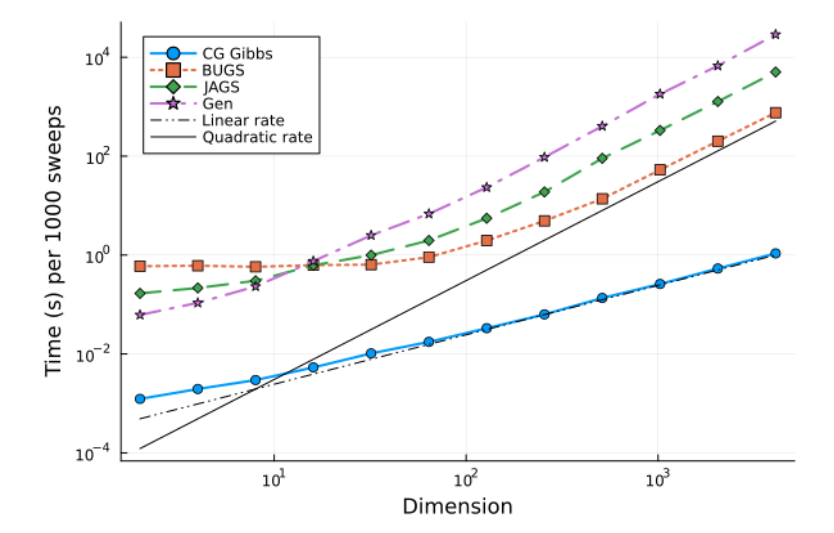
\includegraphics[width=\linewidth,height=0.65\textheight,keepaspectratio]{figure3_runtime.png}
    \end{column}
    \begin{column}{0.32\textwidth}
      \small
      Синтетическая логистическая регрессия,
      $\theta_j\sim\mathcal{N}(0,10^2)$.
      \medskip

      \textbf{По горизонтали:} число параметров $d$.
      \medskip

      \textbf{По вертикали:} секунды на 1000 проходов; меньше --- лучше.
      \medskip

      Обе шкалы логарифмические.
    \end{column}
  \end{columns}
  \medskip
  \textbf{Результат:} CGGibbs близок к $O(d)$; MultiBUGS, JAGS и Gen.jl --- к $O(d^2)$.
\end{frame}

\begin{frame}{Эксперимент 2: реальные задачи классификации}
  \begin{center}
    \begin{tabular}{lrrl}
      \toprule
      Пример & $n$ & Число признаков & Приложение \\
      \midrule
      colon & 62 & 2\,000 & Экспрессия генов \\
      GLI\_85 & 85 & 22\,283 & Экспрессия генов \\
      BASEHOCK & 1\,993 & 4\,862 & Тексты \\
      gisette & 7\,000 & 5\,000 & Распознавание цифр \\
      \bottomrule
    \end{tabular}
  \end{center}
  \begin{block}{Результат}
    CGGibbs эффективнее Stan NUTS на 11 из 12 наборов,
    в лучшем случае ускорение по времени на ESS --- порядка $300\times$.
  \end{block}
\end{frame}

\begin{frame}{Пример colon: преимущество зависит от размерности}
  \begin{columns}[c,onlytextwidth]
    \begin{column}{0.64\textwidth}
      \centering
      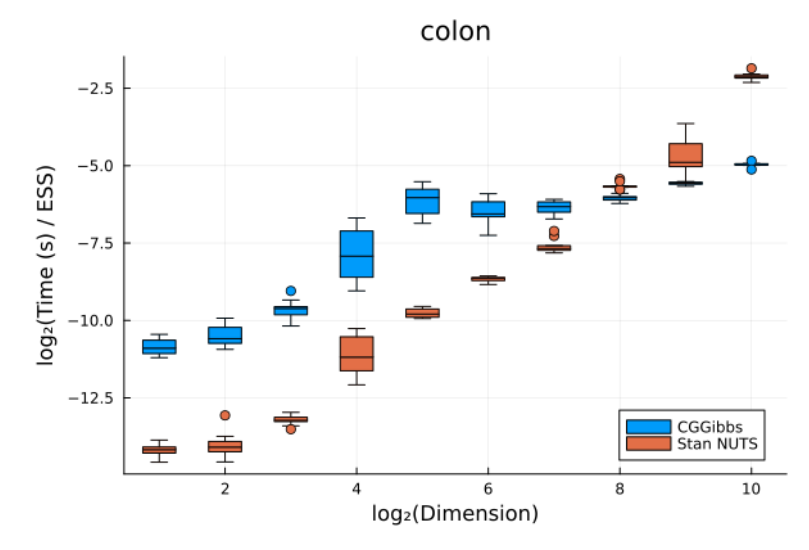
\includegraphics[width=\linewidth,height=0.65\textheight,keepaspectratio]{figure4_colon_ess.png}
    \end{column}
    \begin{column}{0.33\textwidth}
      \small
      $x$: $\log_2 d$.
      \medskip

      $y$: $\log_2$(секунды на ESS); \textbf{меньше --- лучше}.
      \medskip
      
      Время адаптации исключено.
    \end{column}
  \end{columns}
  \medskip
  \textbf{Результат:} NUTS быстрее при малом $d$; при большом $d$ выигрывает CGGibbs.
\end{frame}

\begin{frame}{Итог}
  \begin{enumerate}
    \item Кэш $X\theta$ снижает стоимость прохода Gibbs:
      $O(nd^2)\rightarrow O(nd)$.
    \item Для эффективности важны и размерность, и остаточная обусловленность.
    \item CGGibbs убедителен в высокоразмерных GLM, универсального победителя нет.
  \end{enumerate}
  \medskip
  \begin{block}{Статья-источник}
    \small Son Luu, Zuheng Xu, Nikola Surjanovic, Miguel Biron-Lattes,
    Trevor Campbell, Alexandre Bouchard-Côté.\\
    \textit{Is Gibbs sampling faster than Hamiltonian Monte Carlo on GLMs?}
    \href{https://arxiv.org/abs/2410.03630}{\texttt{arxiv.org/abs/2410.03630}}
  \end{block}
\end{frame}

\end{document}
